\documentclass{article}

\usepackage{graphicx}
\usepackage{hyperref}
\usepackage{tikz}
\usepackage{pgfplots}
\usepackage{multicol}


\author{Rotariu Vlad-Anton}
\title{Minimizări de funcții.\\Hill Climbing. Simulated Annealing.}

\begin{document}
\maketitle

\section{Introducere}
Optimizarea matematică înseamnă selecția celui mai bun element dintr-un set de alternative valabile. Problemele de optimizare apar în discipline precum informatică, inginerie, economie.Optimizarea constă in maximizarea sau minimizarea unei funcții reale, prin alegerea sistematică a parametrilor și calcularea funcției.

In acest articol vor fi prezentați doi algoritmi de optimizare: Hill Climbing si Simulated Annealing impreuna cu implementarea lor in Python.

\section{Algoritmi}
\subsection{Hill Climbing}
Acest algoritm încearca să minimizeze sau să maximizeze o funcție $f(x)$, unde $x$ este un vector de valori. La fiecare iterație, Hill Climbing va adapta un singur element din $x$ și va determina dacă noul vector $x'$ îmbunătățește valoarea lui $f(x)$, caz în care $x := x'$. Algoritmul se încheie în cazul in care nu se găsește niciun $x'$. $f(x)$ se va numi \textbf{minim local}.
\subsection*{Pseudocod}
\begin{tabbing}
t := 0\\
initialize best\\
repeat \=\\
\>  local := FALSE\\
\>  select a candidate solution vc at random\\
\>  evaluate vc\\
\>  repeat \=\\
\>\>    vn := Improve(Neighborhood(vc))\\
\>\> 	if eval(vn) is better than eval(vc)\\
\>\>	then vc := vn\\
\>\>	else local := TRUE\\
\>  until local\\
\>  t := t + 1\\
\>  if vc is better than best\\
\>  then best := vc\\
until t = MAX\\

\end{tabbing}

Se poate observa că pentru a mări spațiul de căutare, algoritmul Hill Climbing este iterat de $t$ ori. Aceste iterații ajuta algoritmul să nu rămână blocat 
într-un minim local. 

In imaginile de mai jos putem observa acest fenomen. Punctele albastre sunt valorile alese de algoritm iar punctele verzi sunt rezultatele unei iteratii. Se observa ca in imaginea din stanga obtinem un minim local, pe cand in a doua imagine algoritmul a facut mai multe iteratii si a reusit sa ajunga chiar in punctul de minim global.

\begin{figure}[h!]
\begin{multicols}{2}
    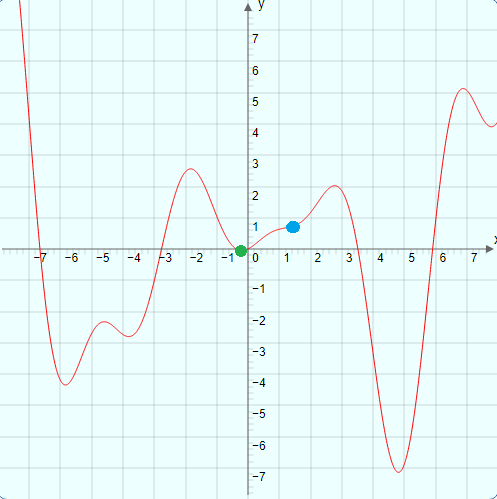
\includegraphics[width=.4\textwidth]{2a}
    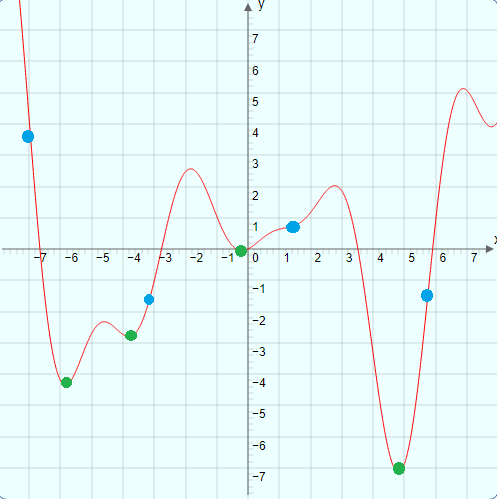
\includegraphics[width=.4\textwidth]{2b}
    \end{multicols}
\end{figure}

\subsection{First improvement și best improvement}
În funcție de metoda în care este implementată funcția $Improve()$\\ există 2 abordări ale algoritmului.
\subsection*{First improvement}
Această abordare este o abordare greedy. Primu vecin bun găsit este ales ca un nou candidat.

\subsection*{Best improvement}
Această abordare presupune faptul ca toți vecinii sunt testați, iar cel mai bun este ales ca un nou candidat.

\subsection{Simulated Annealing}
Numele algoritmului reprezintă o metodă folosită in metalurgie \\(annealing = călire) ce presupune încălzirea și răcirea controlată a materialelor pentru a mări dimensiunea cristalelor și pentru a reduce defectele. Noțiunea de răcire treptată din algoritm este interpretată ca o scădere treptată a probabilității de a accepta soluții mai slabe. Acceptarea acestor soluții permite o căutare mai largă a optimului global.

\subsection*{Iterația}
O iterație a algoritmului presupune:\\\\
1. Alegerea unui vecin $s'$ al unei stări $s$\\
2. Deciderea probabilistică intre a accepta vecinul sau a păstra starea curentă\\\\

Vom alege o funcție $f(x)$. Probabilitatea de acceptare va fi calculată astfel:

$$ P = e^{- \frac{ | f(s) - f(s') |}{T}}, T > 0$$

unde $T$ este temperatura.\\\\

Observăm că $P$ este direct proporțională cu $T$, deci temperatura mare inseamnă probabilitate mare.
\subsection*{Pseudocod}
\begin{tabbing}
t := 0\\
initialize the temperature T\\
select a current candidate solution vc at random\\
evaluate vc\\
repeat \=\\
\>  repeat\=\\
\>\>    select at random vn: a neighbor of vc\\
\>\>    if eval\=(vn) is better than eval(vc)\\
\>\>\>      then vc := vn\\
\>\>\>      else\= if random[0,1) $<$ exp(-abs(eval(vn) - eval(vc)) / T)\\
\>\>\>\>        then vc := vn\\
\>  until (termination-condition)\\
\>  T := g(T; t) \\
\>  t := t + 1\\
until (halting-criterion)
\end{tabbing}

\section{Implementare}
\subsection{Introducere}
Pentru implementarea algoritmilor a fost folosit Python 3.8. Pentru fiecare algoritm a fost creată o clasă aferentă: \texttt{HillClimbing} și \texttt{SimulatedAnnealing}. În constructorul fiecărei clase sunt inițializați următorii membri: \texttt{dimension}(dimensiunea funcției), \texttt{limits}(lista ce contine capetele intervalului funcției), \texttt{function}(funcția de minimizat), \texttt{n}(numărul de iterații), \texttt{precision}(precizia), \texttt{bits\_number}(lungimea necesară reprezentării unei valori ca bitstring).\\\\
în plus, \texttt{HillClimbing} conține membrul \texttt{mode} ce semnifică tipul de algoritm(first sau best).\\\\
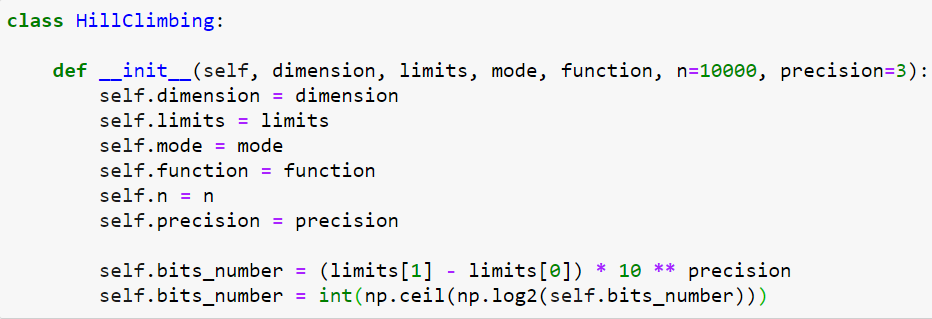
\includegraphics[width=.9\textwidth]{3a}\\
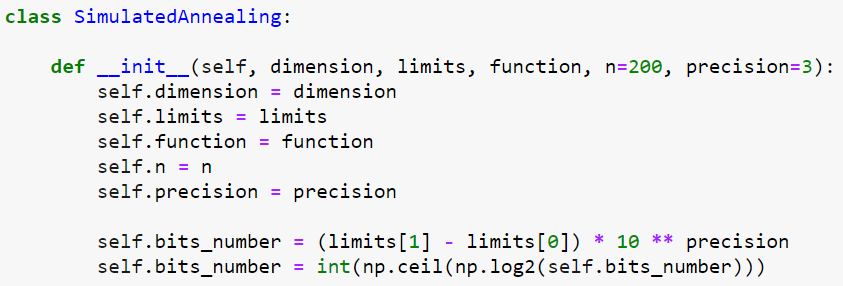
\includegraphics[width=.9\textwidth]{3b}
\subsection{Reprezentarea datelor}
Pentru a reprezenta candidații pentru optimizări, aceștia vor fi transformați in șiruri de biti(bitstring). Intervalul de căutare [a,b] se va discretiza la o precizie $10^{-d}$. Acest interval va fi împărțit în $ N = (b - a) \cdot 10^d$ subintervale, deci sunt necesari $n = [\log_2N]$ biti pentru a reprezenta o valoare din acest interval.\\\\ Formula folosită pentru decodificarea bitstringului este:
$$x = a + decimal(bitstring)\cdot\frac{b-a}{2^n - 1}$$\\\\

În programul nostru Python vom folosi funcția \texttt{generate\_candidate()} pentru a genera aleatoriu un bitstring de lungime \texttt{dimension} $\cdot$ \texttt{bits\_number} ce reprezintă vectorul de parametri a funcției de minimizat.\\\\
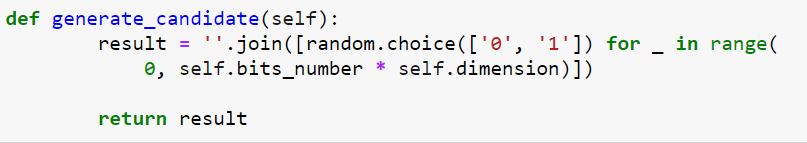
\includegraphics[width=\textwidth]{3c}

\subsection{Căutarea candidaților}
Pentru căutarea noilor candidați(vecinilor), folosim funcția \texttt{mutation()}.Funcția presupune schimbarea bitilor cu ajutorul funcției \texttt{swap\_bit()} pâna când un candidat mai bun este găsit. \texttt{mutation()} este implementată in funcție de algoritmul ales.\\\\
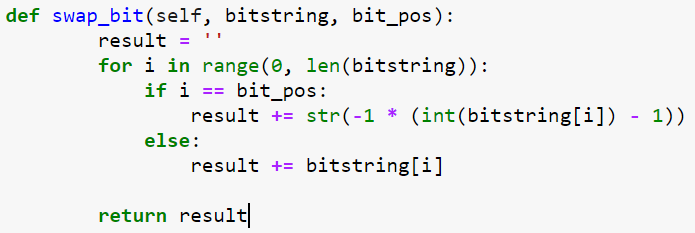
\includegraphics[width=\textwidth]{3f}\\\\
De asemenea pentru a compara candidații, este folosită funcția \texttt{evaluate()} ce decodifică bitstringul in care se afla parametrii si calculează valoarea funcției din \texttt{self.function}.\\\\
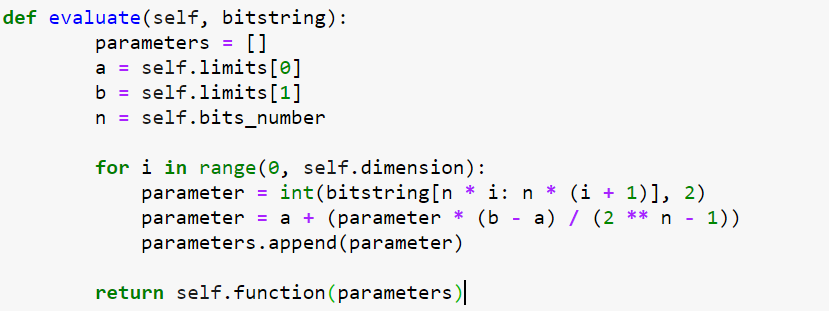
\includegraphics[width=\textwidth]{3g}
\subsection*{Hill Climbing}
Funcția tratează două cazuri, deoarece \texttt{mode} poate fi \textit{first} sau \textit{best}. În primul caz, funcția \texttt{swap\_bit()} este apelată pană este găsit un rezultat mai bun. În al doilea caz, funcția \texttt{swap\_bit()} este apelatț pentru fiecare bit din string, iar cel mai bun candidat este returnat.\\\\
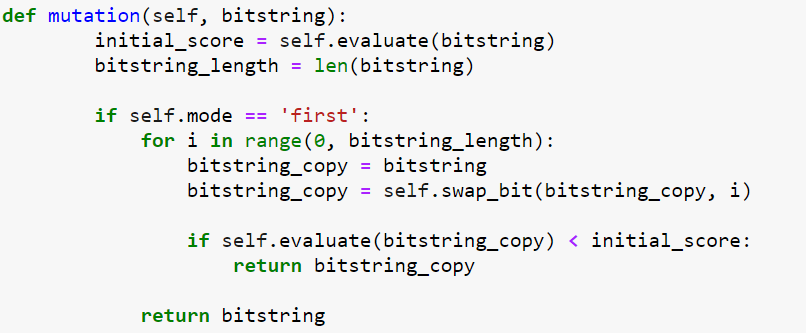
\includegraphics[width=\textwidth]{3d}
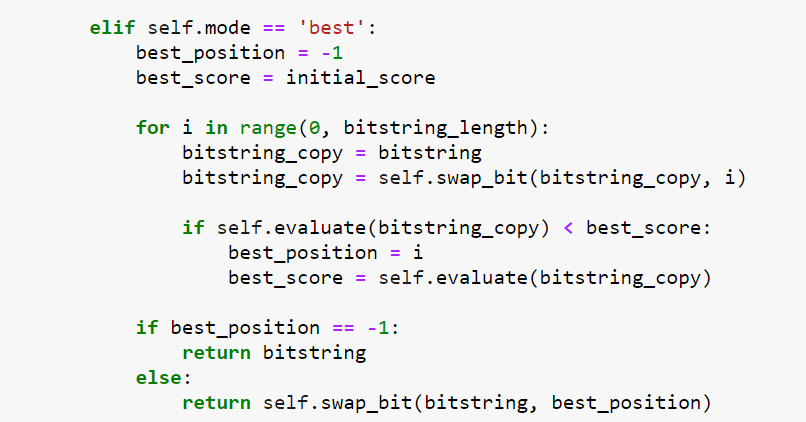
\includegraphics[width=\textwidth]{3e}\\
Se observă ca funcția returnează bitstringul primit ca parametru daca nu gașeste un "vecin" mai bun.
\subsection*{Simulated Annealing}
În acest caz, \texttt{mutation()} schimbă aleatoriu un singur singur bit din bitstring si returnează noul string.\\\\
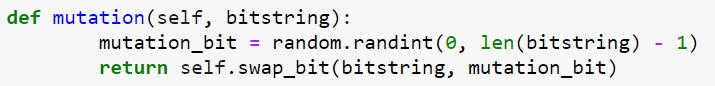
\includegraphics[width=\textwidth]{3h}

\subsection{Iterația}
\subsection*{Hill Climbing}
În funcția \texttt{HC()}, \texttt{search\_minima()} este apelată de \texttt{self.n} ori. \texttt{search\_minima()} generează un prim candidat aleatoriu iar apoi caută "vecini" cu ajutorul funcției \texttt{mutation()}. Dacă "vecinul" este identic cu candidatul, funcția se oprește. \texttt{HC()} returnează cel mai bun rezultat returnat de \texttt{search\_minima()}.\\\\\\\\\\
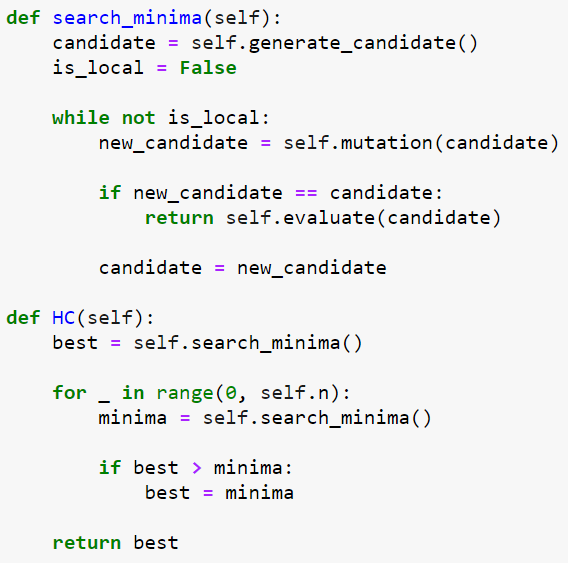
\includegraphics[width=\textwidth]{3i}\\\\

\subsection*{Simulated Annealing}
Funcția \texttt{SA()}, inițializează temperatura si generează "vecini" ai candidatului cu ajutorul funcției \texttt{mutation()}. Candidatul curent va fi schimbat dacă \texttt{evaluate()} returnează o valoare mai buna. De asemenea schimbarea se poate realiza și probabilistic. Funcția se oprește când temperatura atinge un anumit minim.\\\\
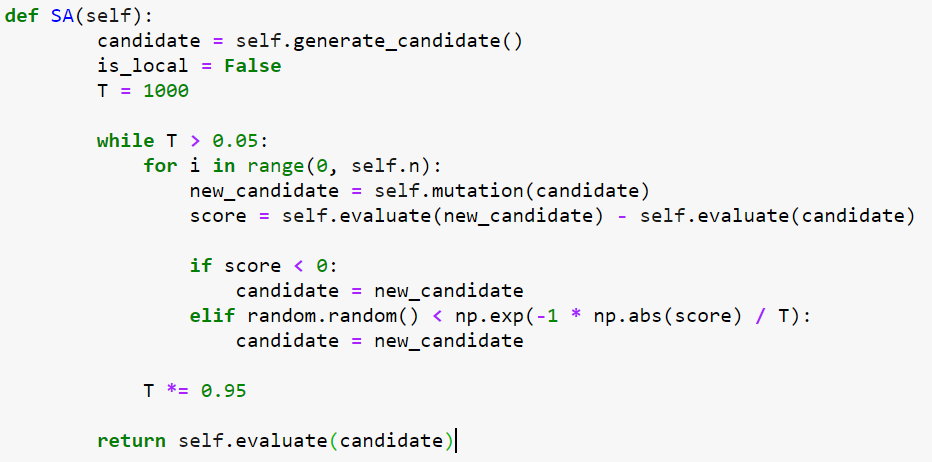
\includegraphics[width=\textwidth]{3j}\\



\section{Experiment}
Pentru acest experiment vom folosi 4 funcții de test. În matematica aplicată, funcțiile de test sunt folositoare pentru a evalua rata convergenței, precizia si performanța generală a algoritmilor de optimizare.\\\\
Funcțiile folosite sunt: \textit{De Jong, Schwefel's, Rastrigin's, Michalewicz's}. Pentru fiecare din aceste funcții vor rula 3 algoritmi: Simulated Annealing, Hill Climbing first si Hill Climbing best.\\\\
De asemenea, algoritmii vor fi rulați pentru mai multe dimensiuni ale funcțiilor: 5, 10, 30.\\\\
(\textit{Algoritmul Hill Climbing a fost rulat pe 200 de iterații iar Simulated Annealing pe 1000 de ițeratii cu un T initial de 1000})\\\\\\\

\subsection*{De Jong}
Funcția De Jong:

$$ f(x) = \sum_{i=1}^n x_i^2, x_i \in [-5.12, 5.12]$$

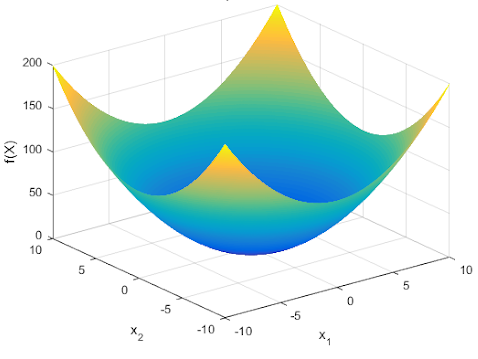
\includegraphics[width=0.7\textwidth]{dejong}\\\\\\
Implementare în Python:\\\\
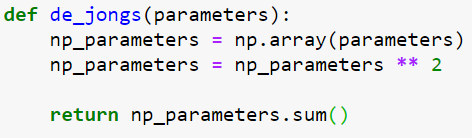
\includegraphics[width=0.7\textwidth]{4a}\\\\\\
Rezultate:\\\\
\begin{tabular}{||c|||l|l|l||}
  \hline
  dimensiune & media & $\sigma$ & timp mediu de execuție(secunde)\\ \hline \hline
  5	  & 0, 0, 0.12 & 0, 0, 0.08 & 14.65, 10.93, 12.51 \\ \hline
  10  & 0, 0, 0.28 & 0, 0, 0.09 & 100,88, 63,68, 14.52 \\ \hline
  30  & 0, 0, 0.71 & 0, 0, 0.17 & 3131, 1772, 39 \\ \hline
\end{tabular}\\\\\\\\
Fiecare valoare din setul de valori obținute corespunde in această ordine unui algoritm: Hill Climbing best, Hill Climbing first, Simulated Annealing.

\subsection*{Schwefel's}
Funcția Schwefel's:

$$  f(x) = - \sum_{i=1}^n - x_i \cdot sin(\sqrt{\left | x_i \right |}), x_i \in \left[ -500, 500 \right]  $$

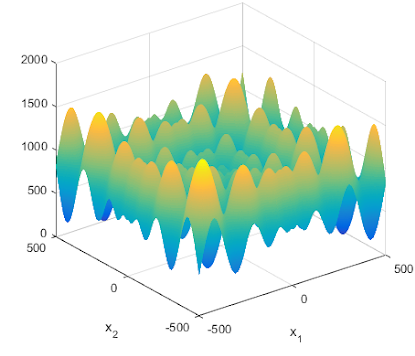
\includegraphics[width=0.7\textwidth]{schwefel}\\\\\\
Implementare în Python:\\\\
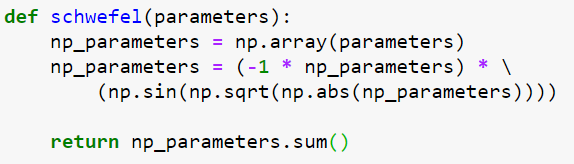
\includegraphics[width=0.7\textwidth]{4b}\\\\\\
Rezultate:\\\\
\begin{tabular}{||c|||l|l|l||}
  \hline
  dimensiune & media & $\sigma$ & timp mediu de execuție(secunde)\\ \hline \hline
  5	  & -2088.10, -2012.42, -2078.70 & 13.47, 42.67, 35.61 & 37.05, 23.74, 15.97 \\ \hline
  10  & -3972.47, -3791.62, -4088.96 & 81.50, 95.21, 99.62 & 226.10, 149.29, 18.52 \\ \hline
  30  & -11136.87, -10600.64, -11842.15 & 175.85, 223.98, 275.26 & 8487.57, 5153.03, 55.05 \\ \hline
\end{tabular}\\\\\\
Fiecare valoare din setul de valori obținute corespunde in această ordine unui algoritm: Hill Climbing best, Hill Climbing first, Simulated Annealing.

\subsection*{Rastrigin's}
Funcția Rastrigin's:

$$ f(x) = A \cdot n + \sum_{i=1}^n \left[ x_i^2 - A \cdot cos(2 \pi x_i) \right],
A = 10, x_i \in \left[ -5.12, 5.15 \right]$$

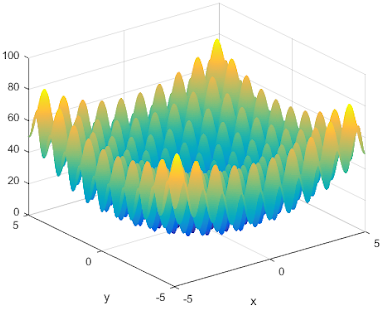
\includegraphics[width=0.7\textwidth]{rastrigin}\\\\\\
Implementare în Python:\\\\
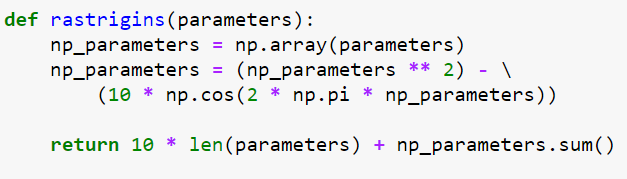
\includegraphics[width=0.7\textwidth]{4c}\\\\\\
Rezultate:\\\\
\begin{tabular}{||c|||l|l|l||}
  \hline
  dimensiune & media & $\sigma$ & timp mediu de execuție(secunde)\\ \hline \hline
  5	  & 1.19, 1.66, 3.65 & 0.60, 0.70, 2.25 & 15.81, 10.66, 15.60 \\ \hline
  10  & 5.80, 7.14, 9.00 & 1.31, 1.73, 3.52 & 89.07, 59.86, 17.12 \\ \hline
  30  & 32.37, 39.96, 31.89 & 3.31, 3.11, 5.66 & 2563.94, 1570.71, 42.26 \\ \hline
\end{tabular}\\\\\\
Fiecare valoare din setul de valori obținute corespunde in această ordine unui algoritm: Hill Climbing best, Hill Climbing first, Simulated Annealing.

\subsection*{Michalewicz's}
Funcția Michalewicz's:

$$ f(x) = - \sum_{i=1}^n sin(x_i) \cdot \left(sin\left( \frac{i \cdot x_i^ 2}{\pi} \right)\right)^{2 \cdot m} , m = 10, x_i \in \left[ 0, \pi \right]$$

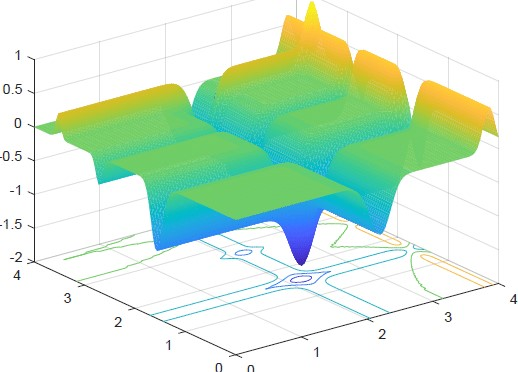
\includegraphics[width=0.7\textwidth]{michalewicz}\\\\\\
Implementare în Python:\\\\
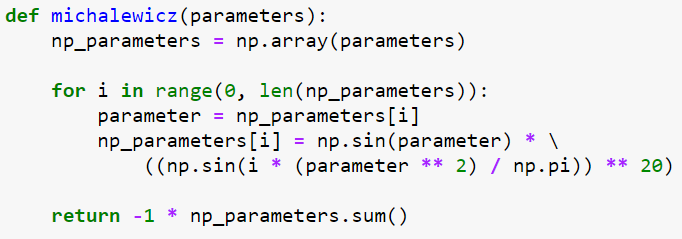
\includegraphics[width=0.7\textwidth]{4d}\\\\\\
Rezultate:\\\\
\begin{tabular}{||c|||l|l|l||}
  \hline
  dimensiune & media & $\sigma$ & timp mediu de execuție(secunde)\\ \hline \hline
  5	  & -3.69, -3.69, -3.52 & 0, 0, 0.13 & 18.20, 13.40, 24.13 \\ \hline
  10  & -8.32, -8.24, -8.00 & 0.08, 0.13, 0.23 & 120.57, 78.45, 34.61 \\ \hline
  30  & -25.75, -24.93, -25.86 & 0.30, 0.32, 0.46 & 3975.52, 1903.29, 90.58 \\ \hline
\end{tabular}\\\\\\\\
Fiecare valoare din setul de valori obținute corespunde în această ordine unui algoritm: Hill Climbing best, Hill Climbing first, Simulated Annealing.

\subsection*{Optimizări}
Pentru a reduce timpul de rulare algoritmii au folosit procese multiple.\\\\
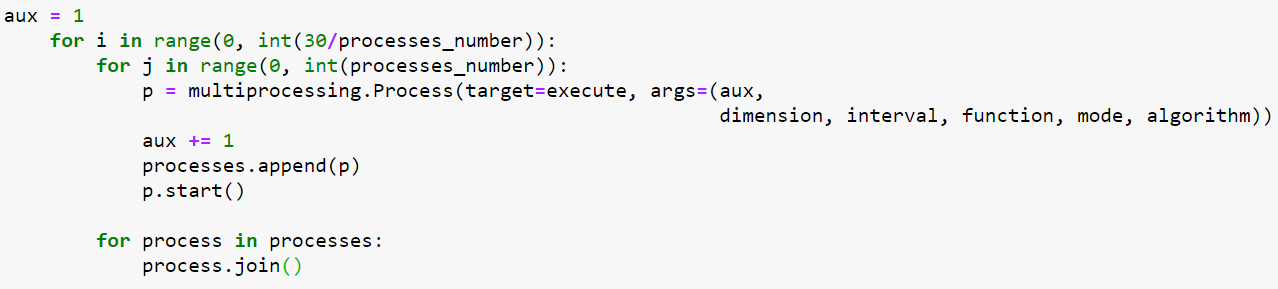
\includegraphics[width=\textwidth]{4e}\\\\
De asemenea pentru a grăbi operațiile ce presupun liste a fost folosită libraria \texttt{numpy}(vezi implementarea funcțiilor).

\section{Concluzii}
Concluziile rezultate din compararea tabelelor de valori sunt următoarele:\\

\begin{enumerate}
 \item Hill Climbing best este cel mai încet algoritm. Pe de altă parte acesta oferă cele mai bune rezultate și cele mai mici deviații standard.
 \item Simulated Annealing este cel mai rapid algoritm, dar nu oferă întotdeauna cele mai bune soluții.
\begin{figure}[h!]
\begin{multicols}{2}
    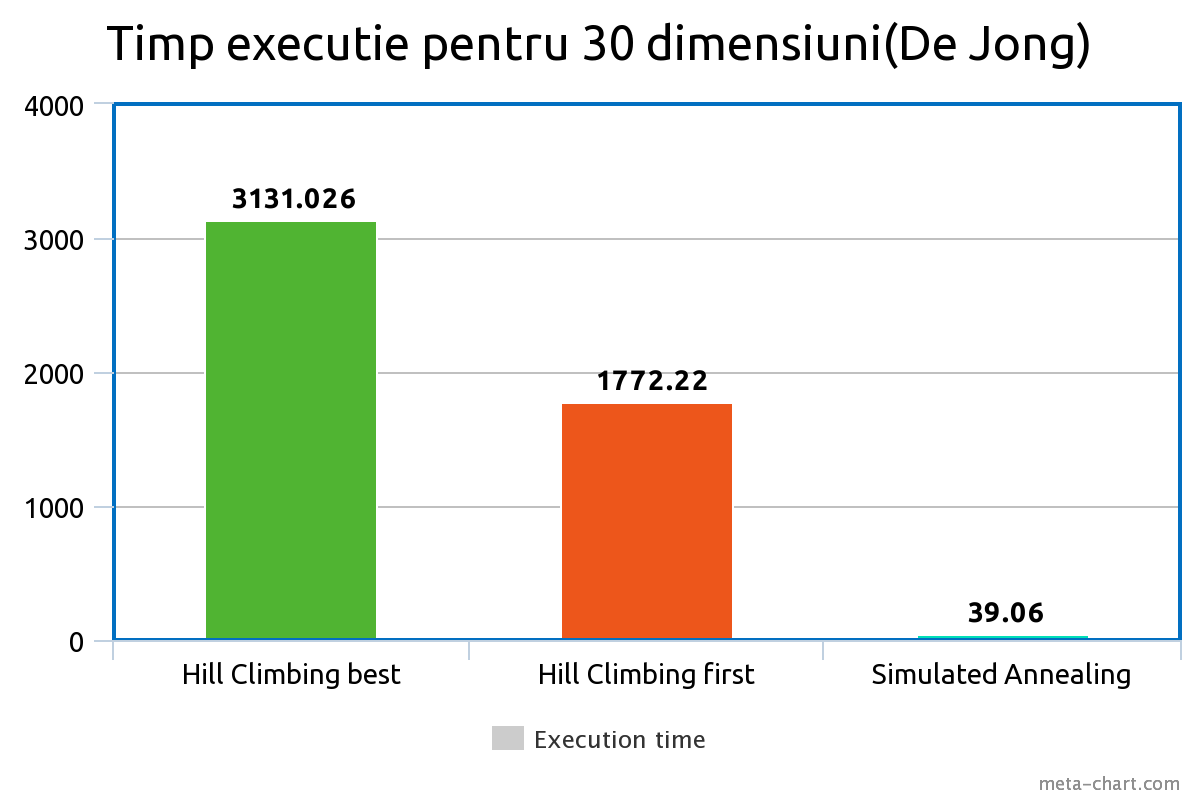
\includegraphics[width=.43\textwidth]{metachart}
    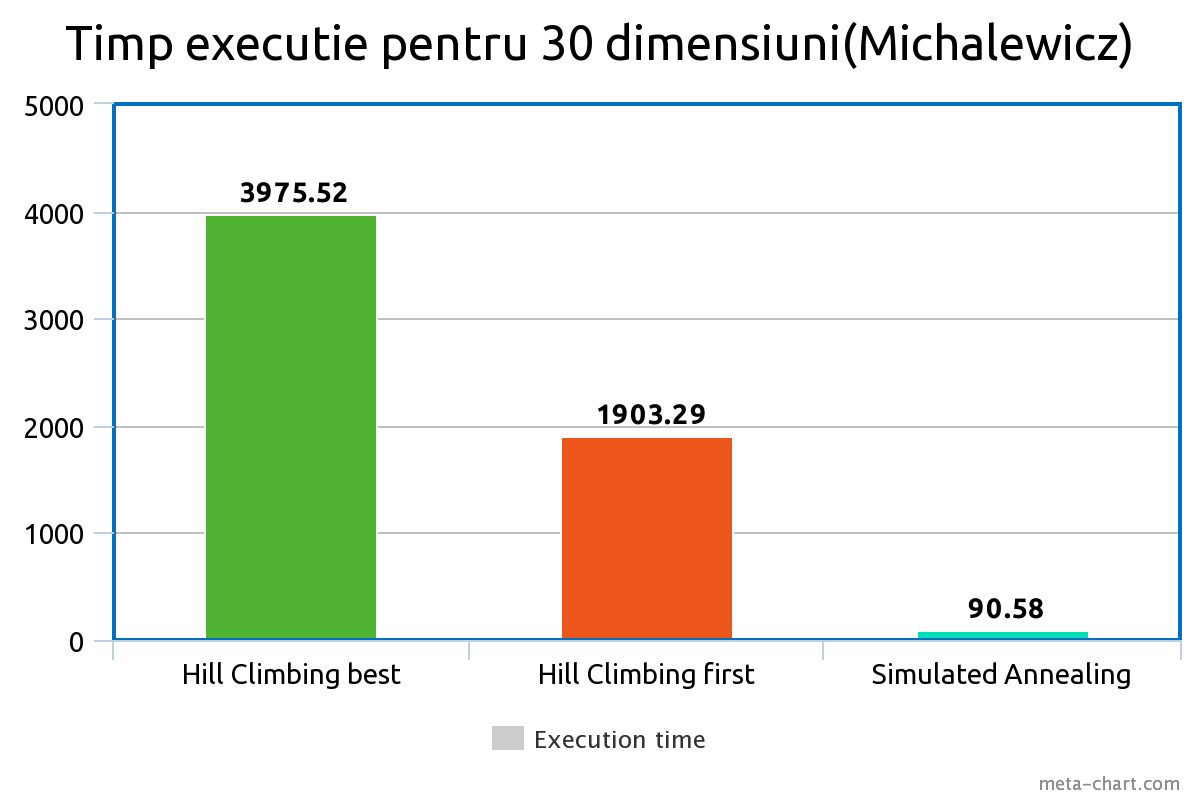
\includegraphics[width=.43\textwidth]{metachart1}
    \end{multicols}
\begin{multicols}{2}
    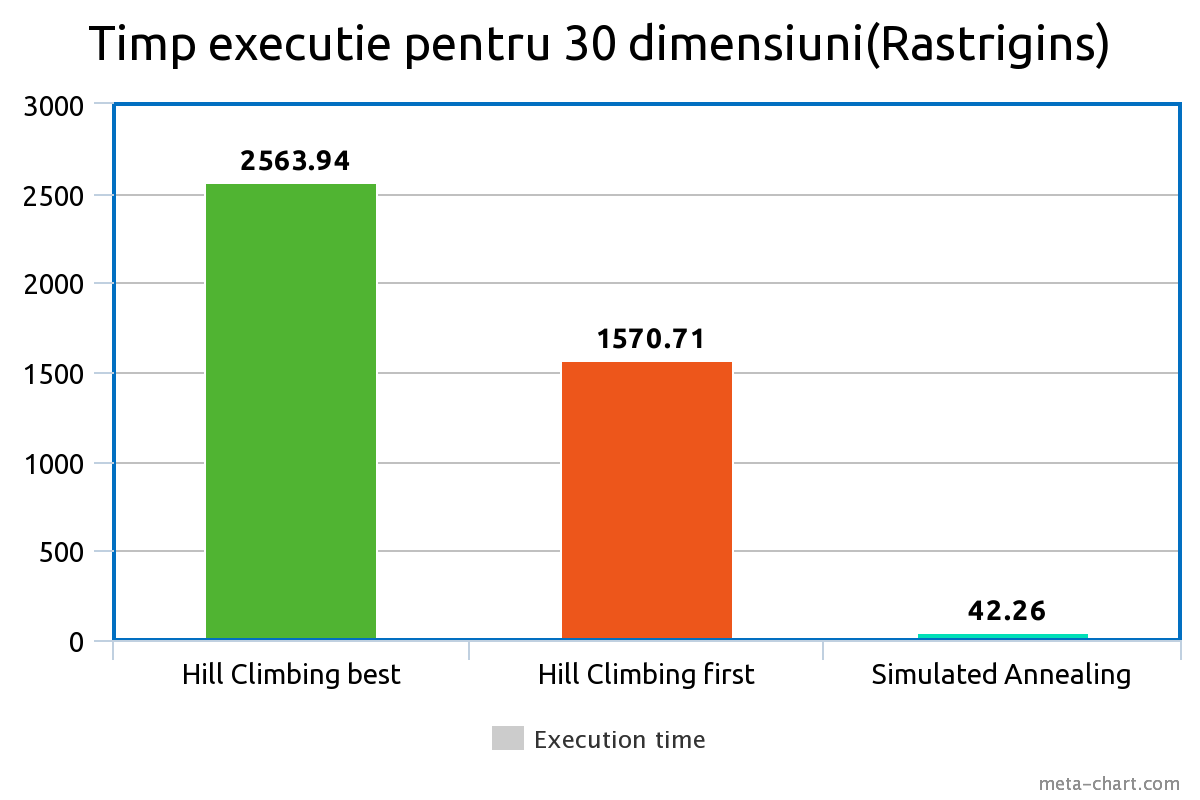
\includegraphics[width=.43\textwidth]{metachart2}
    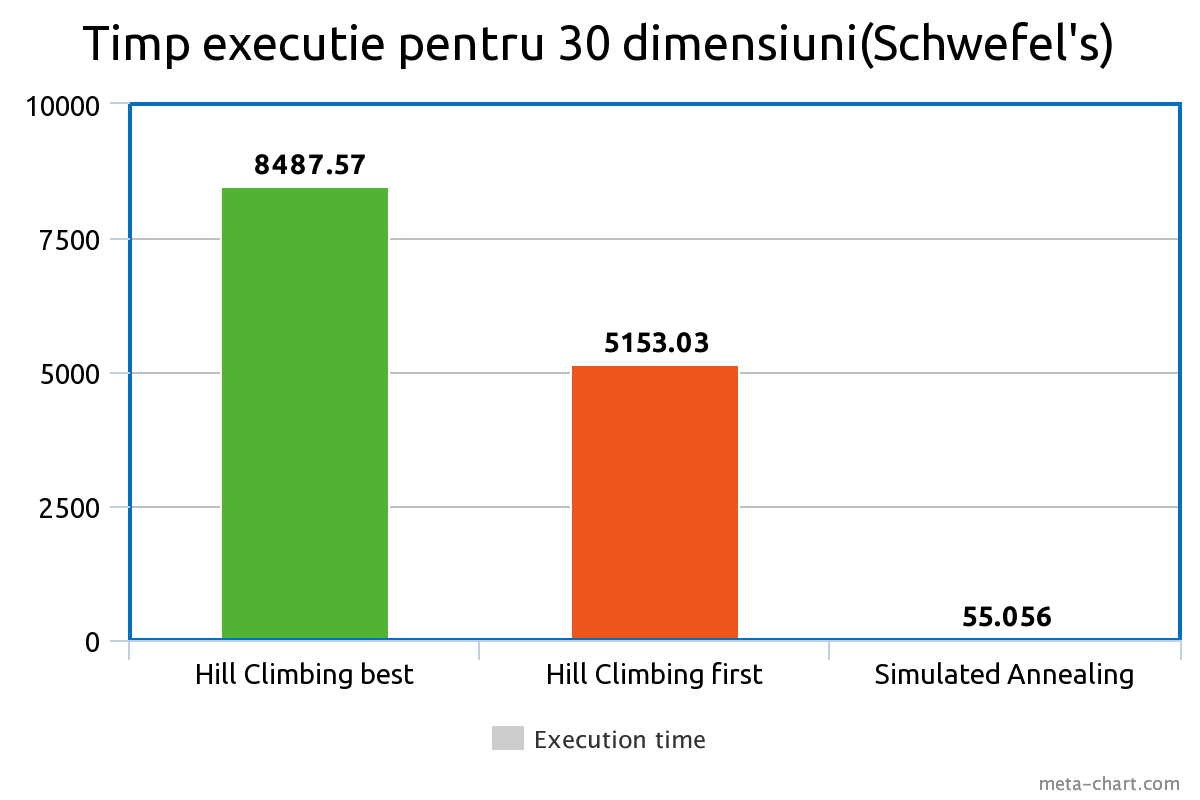
\includegraphics[width=.43\textwidth]{metachart3}
    \end{multicols}
\end{figure}
 \item Timpul de execuție crește exponențial cu numărul de dimensiuni. Putem vizualiza acest lucru pe datele obținute pe algoritmul Hill Climbing best pentru funcția Schwefel cu câte 3 iterații.
 \\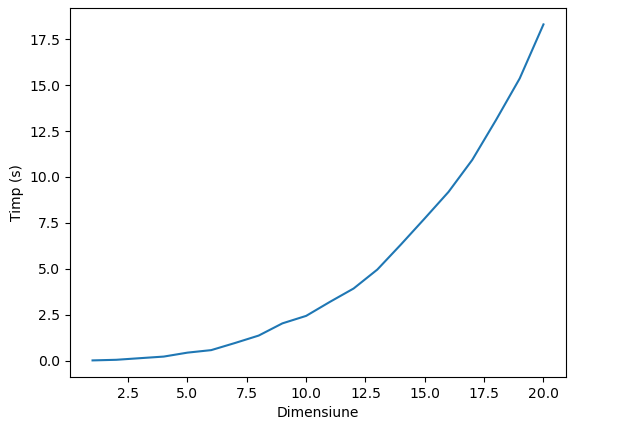
\includegraphics[width=0.6\textwidth]{timeplot}
\end{enumerate}


\begin{thebibliography}{9}
  
\bibitem{wikipedia}
  Wikipedia
  \\ Hill Climbing.
  \url{https://en.wikipedia.org/wiki/Hill_climbing}
  \\ Simulated Annealing.
  \url{https://en.wikipedia.org/wiki/Simulated_annealing}

\bibitem{BenchmarkFcns}
	BenchmarkFcns
	\\ Sphere function.
	\url{http://benchmarkfcns.xyz/benchmarkfcns/spherefcn.html}
	\\ Schwefel function.
	\url{http://benchmarkfcns.xyz/benchmarkfcns/schwefelfcn.html}
	\\ Rastrigin function.
	\url{http://benchmarkfcns.xyz/benchmarkfcns/rastriginfcn.html}
\bibitem{ResearchGate}
	ResearchGate
	\\ Michalewicz function.
	\url{https://www.researchgate.net/figure/The-landscape-of-the-Michalewicz-Function_fig4_339814374} 

\bibitem{GEATbx}
	GEATbx
	\url{http://www.geatbx.com/docu/fcnindex-01.html#P150_6749}
	
\bibitem{Meta-Chart}
	Meta-Chart
	\url{https://www.meta-chart.com/bar}
	
\bibitem{Pandas}
	Pandas
	\url{https://pandas.pydata.org/}
	
\bibitem{Jupyter}
	Jupyter
	\url{https://jupyter.org/}
  
\end{thebibliography}  
\end{document}